\chapter{Improved tolopogical operations}
\label{c:topology}

Throughout this chapter we will refer to various subroutines by what they perform.
\begin{enumerate}
    \item Time evolution: solve the differential equation governing dislocation motion.
    \item Separation: separate high energy, highly connected nodes into lower energy nodes with fewer connections.
    \item Collision detection: detect collisions between segments, i.e. which segments collide, where they collide, what nodes are involved.
    \item Collision resolution: resolve collisions between segments, i.e. where they collide, what nodes to merge and where to do so.
    \item Remeshing: ensuring the network has the appropriate resolution. Broken into 3 main parts:
          \begin{enumerate}
              \item Virtual: nodes that have exited the finite volume need to be tracked so the slip step displacements can be properly accounted for. Virtual-surface segments, and virtual-virual segments are considered external and do not interact with internal segments in any way.
              \item Surface: segments that exit the finite volume need a node on the surface to keep track of where they connect to the internal network. Surface-internal nodes are considered internal, so they interact with other internal segments.
              \item Internal: nodes that are internal to the finite volume.
          \end{enumerate}
\end{enumerate}

\section{Introduction}

In 2D, dislocations are parametrised as points on a surface. Therefore, aside from annihilation, interactions with grain boundaries \cite{grain_size_eff1, grain_size_eff2}, and perhaps the creation of superdislocations, topological changes in the dislocation network can be mostly ignored. However, in 3D, dislocations are parametrised as lines in a volume. This gives rise to extra complexities that result from multiple dislocations coming into contact with one another. These reactions ultimately lead to the formation of many secondary structures with their own properties that affect the rest of the network.

The local dislocation density at these interaction sites, particularly arround sessile (immobile) junctions, tends to increase with time. Therefore, so do the local stress gradients, and with increasing stress gradients come increasing velocity gradients, which lead to global decreases in timestep. But a smaller timestep is not the only consequence, increases in dislocation density also mean higher probabilities of dislocation-dislocation interactions, so the phenomenon is autocatalytic and self-perpetuating. So properly accounting for these changes is of the utmost importance, particularly for simulations with high dislocation densities such as nanoindentation. This chapter details these improvements.

\section{Non-commutativity of topological changes}\label{s:nonCommutativity}

For a given iteration, the time-evolution and topological changes used to be performed in the following order:
\begin{enumerate}
    \item time-evolution,
    \item separate highly connected nodes,
    \item detect and resolve collisions, and
    \item remesh network.
\end{enumerate}
This ordering was problematic. Fundamentally, it means the time evolution erroneously accounts for complex structures that should have dissipated into lower energy ones as per the quasi-static principle the model is based on. In other words, detecting and resolving collisions, generates highly connected structures that are high energy and thus produce large local stress gradients. The assumption that a node and its neighbours experience similar conditions breaks down near highly connected nodes. Moreover, the assmumption that the network is at thermodynamic equilibrium at every time step breaks down when there are highly connected nodes that would otherwise be broken up by separation. Both of these lead to \cref{eq:nodeVel} not holding, which is the fundamental assumption behind our mobility laws.

Moreover, the order in which topological changes were carried out was also very sub-optimal from a practical aspect. Colliding after separating would sometimes result in nodes being separated only to immediately collide again. Remeshing only at the end meant the input network for the topological operations could have contained segments whose lengths were outside the bounds defined by the input file. Meaning the network may not have been properly discretised, leading to unecessarily complex structures that may not have had the required resolution. The solution was to simply remesh the network after its time evolution and before topological functions.

The other problem with this ordering was the combinatorial complexity of the separation subroutine. The consequence of the old ordering is that as simulations advanced, collisions tend to become more common. A higher collision rate means more highly connected nodes. The role of separation is to break these high energy, highly connected nodes into lower energy nodes with fewer connections. However, splitting nodes is a combinatorial problem, so the gross computational complexity is functionally $\mathcal{O}(N!)$, which is pretty much the worst possible scaling barring special cases such as tetration. \Cref{s:separation} contains a more detailed explanation as well as resolution of the problem.

Aside from the order of operations, a very large number of changes, fixes and improvements needed to be made to practically all topological operations. Here we detail only the ones this project had a major hand in fixing, namely collision detection and resolution, separation, and part of the surface remeshing. The rest were led by Bruce Bromage as part of his project, and the one preventing the formation of superdislocations by Haiyang Yu.

The end result of all this work is the new order of operations:
\begin{enumerate}
    \item time-evolution,
    \item remesh,
    \item collision detection and resolution + separation loop,
    \item mobilise highly connected immobile nodes,
    \item separate highly connected nodes,
    \item remesh.
\end{enumerate}
This ensures the time evolution and topological functions are all fed a network that is as clean and well-resolved as the input parameters say it should be. Although this incurs a computational cost, the benefits of having a cleaner network for the other functions to work with vastly outweigh the increased cost of calling the cheap remeshing subroutine more times.

\section{Collision}\label{s:collision}

\subsection{Hinges}\label{ss:hinges}

The lowest hanging fruit and most obvious problem were collisions that share a lot of similarities with the remeshing criteria that checks for a minimum area enclosed between two segments connected by a single node, which we call \emph{hinges}, as shown in \cref{f:hinge}. A single dislocation hinge can lead to three final topologies (two of which are degenerate). The conditions for which can be simultaneously met in any combination:
\begin{enumerate}
    \item Remeshing to eliminate the middle node because the area, $a$, enclosed by the triangle created by segments $s_1$ and $s_2$ is less than the minimum allowable area, $a_{\rvar{min}}$.
    \item Colliding $s_1$ into $s_2$ if the minimum distance, $l_1$, between the non-hinge node of $s_1$ (the node $s_1$ does not share with $s_2$) and segment $s_2$ is less than the collision distance, $l_1 < l_{\rvar{col}}$.
    \item Colliding $s_2$ into $s_1$ if the minimum distance, $l_2$, between the non-hinge node of $s_2$ and segment $s_1$ is less than the collision distance, $l_2 < l_{\rvar{col}}$.
\end{enumerate}
\begin{figure}
    \centering
    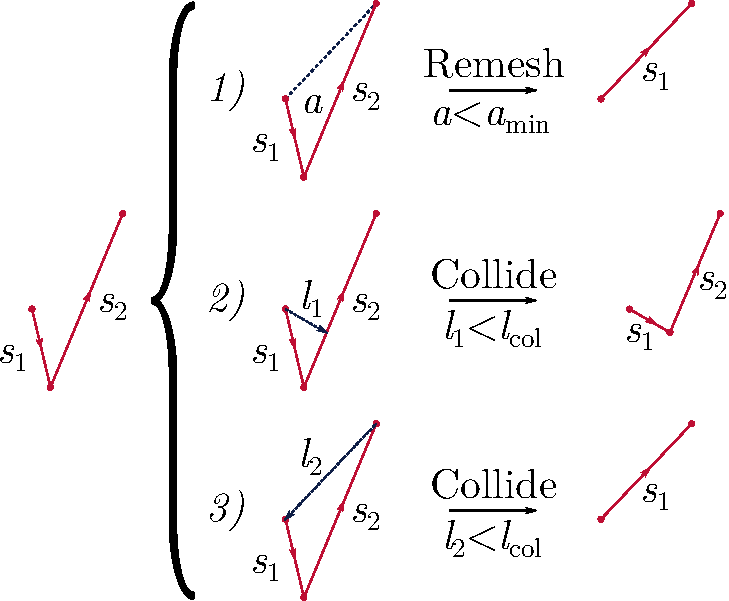
\includegraphics[width=0.7\linewidth]{hinge.pdf}
    \caption[A single dislocation hinge can lead to three different final topologies.]{A single dislocation hinge can lead to three final topologies (two of which are degenerate), the conditions for which can be simultaneously met in any combination. Where $a$ is the enclosed area, $l_1$ and $l_2$ are possible minimum lengths between both segments.}
    \label{f:hinge}
\end{figure}

The combination in which the conditions can be met, and the order in which they are checked could have drastic downstream consequences (see \cref{s:nonCommutativity}), \emph{especially} at high dislocation densities where multiple collisions happen at every timestep. This had not been an issue prior to many of the improvements made to the codebase, but with the increased ability to model a larger number of dislocations to a sufficiently advanced point where this was having a significant impact, particularly in Haiyang Yu's nanoindentation simulations, which would either go wrong by creating unphysical junctions and/or massively slow down after reaching a certain point.

This was a multi-stage fix, where each fix progressively uncovered more and more shortcomings resulting from the unavoidable coupling between topological operations. These progressive fixes are detailed in \cref{s:nonCommutativity}. Here we will only focus on problems with collisions.

The first fix involved prioritising hinge collisions above the other type of collision, which we call \emph{two-line} collision. This meant detecting and resolving all possible hinge collisions before detecting and resolving any two-line collision. The rationale behind this is that segments in a hinge are already part of a single dislocation line. Because they are connected to each other at a single hinge node, they are already interacting via line tension and remote interaction; whereas two unconnected segments approaching one another only interact via remote interaction. The other, more practical advantage of resolving hinges first is that hinge collisions decrease the total segment length of the involved segments, therefore reducing their collision radii and the probability of them colliding with other segments via two-line collisions.

The second was much more subtle. \Cref{f:hinge} has two options for colliding a hinge, as seen in \cref{f:hinge}. Both resulting in different topologies. Which topology we ended up with was down to which segment, $s_1$ or $s_2$, the code came across first. If $s_1$ was first, then the answer would be $2)$, otherwise it would be $3)$. At the very least, the answer should be the same for a given network topology, regardless of how it is represented. So we decided to ensure the distance calculated was always the minimum out of both scenarios. Which means the distance calculated should be the minumum distance between the non-hinge node of the short segment, to the long segment. There is an argument to be made that the solution should be the other way round, as that would ensure the final structure has the minimum total length, as well as one less node. However, this could potentially leave many hinges around that would have otherwise been resolved.

\subsection{Collision distance}\label{ss:collisionDistance}

In the same vein as \cref{ss:hinges}, two-line collisions were being improperly prioritised. They occurred arbitrarily as the code came across them. Again yielding different answers for different representations of the same network. Only this time it had to do with the collision radius, as shown in \cref{f:collisionRadius}.
\begin{figure}
    \centering
    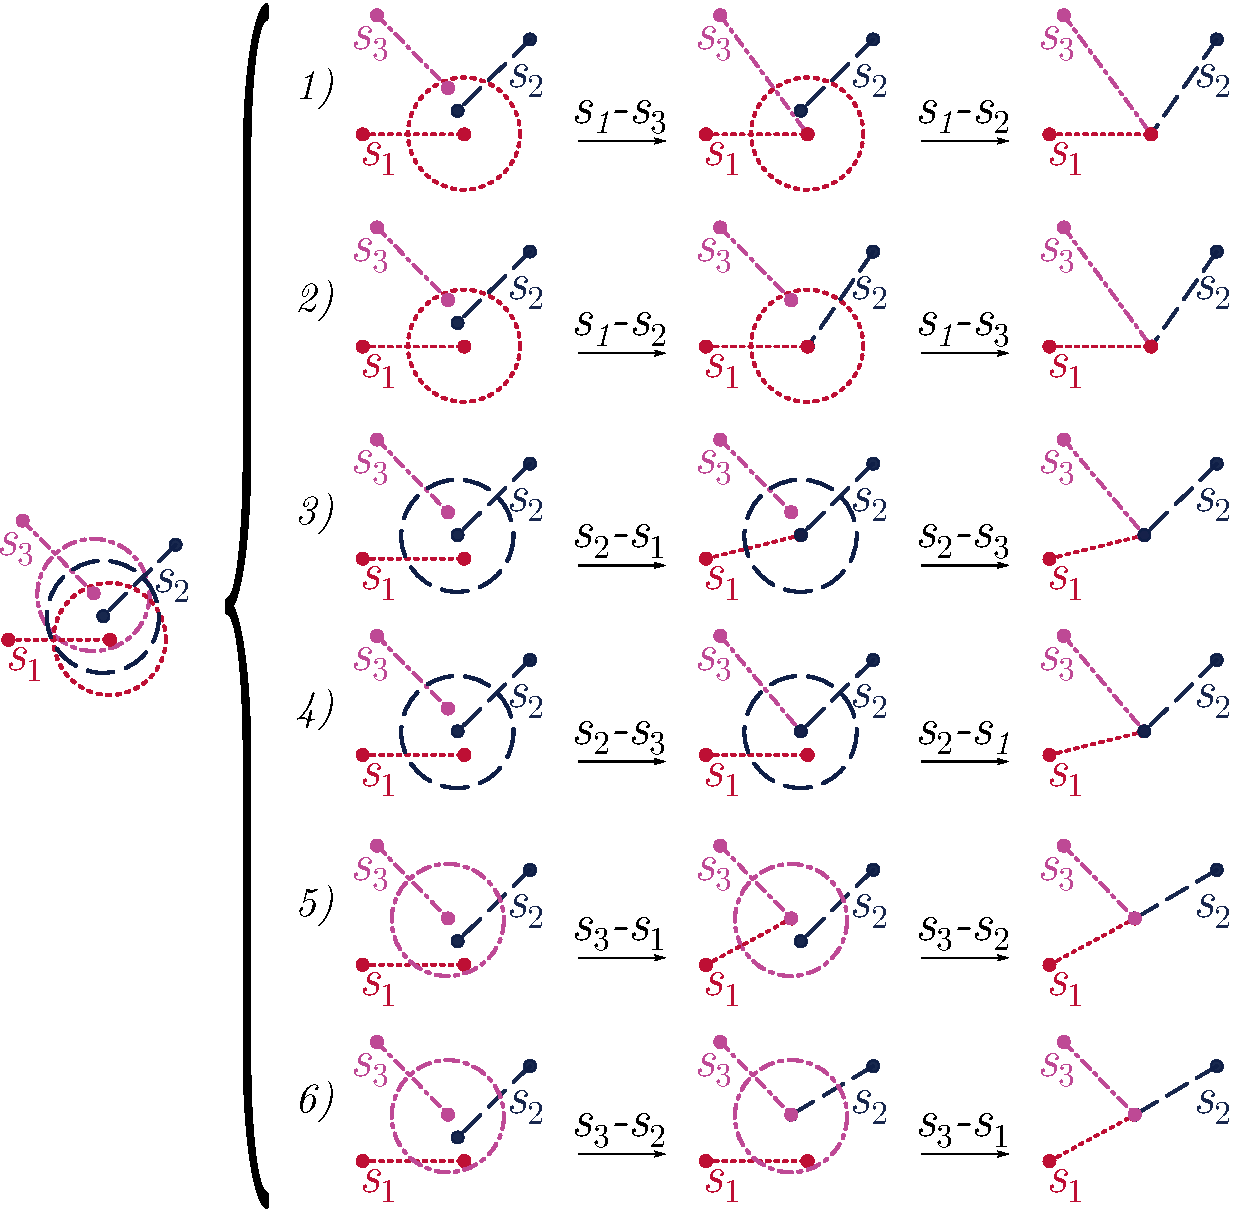
\includegraphics[width=0.9\linewidth]{collisionDist.pdf}
    \caption[Dislocation segments inside different collision radii.]{Multiple dislocation segments inside the same collision radius. Resolving all collisions at once leads to 3 different structures, 6 total but half are degenerate. Circles represent collision radii for the segments with corresponding line style and colour.}
    \label{f:collisionRadius}
\end{figure}

The actual algorithm is more sophisticated because it accounts for whole segments, as well as their relative velocities. It returns the points along the segments that minimise the distance between segments. These points are then used to decide which nodes to merge and how to do so.

The problem was that as soon as a viable collision was found, the function returned. So in a scenario like \cref{f:collisionRadius}, if the code was looking for a collision on $s_1$, and it came across $s_3$ first, it would flag that as the collision, disregarding the fact that not only was $s_2$ closer, but $s_2$ and $s_3$ are also closer; and perhaps the true minimal distance was not even between $s_1$ and another segment, but between $s_2$ and $s_3$. We had to apply the same fix to hinge collisions. Admittedly, it matters less in that case as they tend to be rarer, plus their size is limited anyway, but still ensures a more correct solution.

The original algorithm had $\mathcal{O}(N^2)$, $\Theta(N^2/4)$ and $\Omega(1)$ for its upper, average, and lower asymptotic bounds\footnote{The original collision detection algorithm had these three asymptotic bounds because it returned as soon as it found a single collision. $\mathcal{O}(N^2)$ when no collision was found, as it had to check all segment-segment interactions. $\Theta(N^2/4)$ because on average, it would have had to traverse half the segments to find $s_1$ and half the segments again to find $s_2$. The absolute best performance would be $\mathcal{O}(1)$, where the colliding segments are the first two segments in the list.} respectively for fixed $N$, where $N$ is the number of segments. The new one is always $\mathcal{O}(N^2)$. However, $N^2/4 \to N^2$ as $N\to\infty$, so as simulations grow larger, the performance hit gets lower. Moreover, the algorithm is quite cheap compared to other processes, and the improved accuracy is very much worth the small cost.

Better collision detection tends to result in faster simulations because the resulting structures are guaranteed to produce the shortest segments and therefore more accurate junctions. Shorter segments can also be cleaned up by remeshing if they meet the remeshing criteria. Referring back to \cref{f:collisionRadius}, it is evident that the structure formed by colliding $s_1$ and $s_3$ is higher energy than that formed by colliding $s_1$ and $s_2$. In this case, if we fully resolve the two possible collisions for every combination of segments, we arrive at three different scenarios (6 total, but half are degenerate). However, this still leaves room for producing different answers given different representations of the network. If, for example the most appropriate collision is $s_2$-$s_3$ (cases 4 and 6 in \cref{f:collisionRadius}), the order in which it is performed can yield two slightly different structures after resolving the remaining collisions. However, this is preferrable over finding other, less favourable collisions that may lead to unecessarily complex structures.

We must also bear in mind that \cref{f:collisionRadius} shows a minimal example for a case where three collision radii overlap, and the resulting structures are not dissimilar to one another. In fact, if the final junction formed is glissile, they should evolve similarly. However, as the code was now able to handle and evolve larger numbers of dislocations further than before, it became apparent that the collision algorithms needed to be improved. After all, as the number of candidate collisions increased, so did the chance for the code to pick the wrong one and for that to have a deleterious effect on the code.

\section{Separation}\label{s:separation}

One of the larger problems with high dislocation densities, is the computational complexity of the separation function. Its role is to take high energy, highly connected structures and break them apart into lower energy, lower connection ones. The separation criteria is the power dissipation of the split configuration, compared to the power dissipation of the unseparated structure. The power dissipation is given by,
\begin{align}\label{eq:powerDiss}
    P_m & = \sum\limits_i^N\vec{v}_i \cdot \vec{f}_i\,,
\end{align}
where $P_m$ is the power dissipation of splitting mode $m$, $\vec{v}_i$ is nodal velocity, and $\vec{f}_i$ the nodal force of node $i$ participating in the splitting mode. Locality is assumed, so the computation of the pre-separation---reference---power dissipation involves only the node to be separated ($N=1$); whereas the computation of the post-separation power dissipation involves the two nodes the node splits into ($N=2$). The splitting mode chosen by the separation subroutine is that which dissipates the largest amount of power. If the pre-separation node has a higher power dissipation than any separation mode, it remains unseparated. In practice, the reference power dissipation is multiplied by a factor 1.05 to prevent nodes from flickering between being separated and colliding over multiple timesteps until the nodes can move far enough apart that they no longer collide.

Separation is a very poorly scaling operation. For a single multi-connected node we have,
\begin{align}
    M & = \sum\limits_{j=2}^{\left\lfloor C/2 \right\rfloor} \binom{C}{j} \coloneqq \sum\limits_{j=2}^{\left\lfloor C/2 \right\rfloor} \dfrac{C!}{(C-j)! j!}\,.
\end{align}
Where $C$ is the number of connections a node has, $j$ the number of connections in a splitting mode\footnote{This is the number of connections taken by one node after the split, the other would retain $C-j$ connections.}, and $M$ is the total number of splitting modes. Mirror symmetries where $C = 2j$ half the number of possible splitting configurations in those cases. This type of scaling leads to a combinatorial explotion in computational complexity at higher connectivities. At best, this puts the lower bound at approximately Sterling's factorial formula $N! \approx \Omega(N\log{N})$ for large $N$. Furthermore, all of these configurations must be generated---an $\mathcal{O}(M)$ operation, where $M$ are the number of nodes to be added---in order to check their power dissipation. Unfortunately, this is a relatively expensive operation because the code dynamically expands the relevant arrays. The nodal velocities and segment forces must then be calcualted for every configuration. Whichever has the largest energy dissipation---provided it is higher than the reference configuration---is picked as the final configuration. Since locality is assumed, only the forces and mobilities of the nodes and segments directly involved in the split are accounted for, however this still involves an $\mathcal{O}(2 N)$ call to the remote force calculation per splitting mode. Since the procedure must be performed for all nodes exceeding the maximum allowed connectivity, it is extremely important that individual nodal connectivities as well as, the total number of highly connected nodes, remain as low as possible.

The solution may appear to be as simple as calling separation after resolving a single collision. Then looping through all collisions in a given timestep. However, this can cause collisions to be undone, leading to an infinite loop. Solving this was a long, multi-stage process. However, the solution is rather simple and elegant. We simply applied the power dissipation criteria to the collision-separation loop as described by \cref{alg:collisionSep}.
\begin{algorithm}
    \caption{Collision-separation algorithm with power dissipation.}
    \label{alg:collisionSep}
    \begin{enumerate}
        \item Set up \texttt{s1Skip} and \texttt{s2Skip}, which are empty buffers for skipping pairs of corresponding segments in the collision detection.
        \item Detect collision, skips corresponding segment pairs in \texttt{s1Skip} and \texttt{s2Skip}. Among the return values are the colliding segments \texttt{s1} and \texttt{s2}.
        \item If no collision was detected, exit collision-separation loop and carry on with the simulation.
        \item If a collision was detected, resolve collision. Among the return values are the pre-collision power dissipation and the node merged into, \texttt{mergednodeid}.
        \item Separate multiply connected nodes, among the return values is the maximum power dissipation post-separation for node \texttt{mergednodeid}. If node \texttt{mergednodeid} is not separated, this value is zero. Otherwise, it is equal to the maximum power dissipation; be it from the unseparated \texttt{mergednodeid}, or the nodes it separated into.
        \item If the power dissipation post-separation is larger than the power dissipation pre-collision, then clear \texttt{s1Skip} and \texttt{s2Skip}, update the network and auxiliary matrices, and return to 2. Else, add \texttt{s1} and \texttt{s2} to \texttt{s1Skip} and \texttt{s2Skip} respectively, don't update the network and auxiliary matrices, and return to 2.
    \end{enumerate}
\end{algorithm}

This can lead to collisions being checked more than once, but in keeping with the quasi-static assumption, ensures the network is always in a first-order minimum energy configuration.\footnote{A true minimal energy structure would require all collisions to be performed at once, and a full, global traversal of every splitting mode tree.}

It is worth noting that nodes labelled as immobile (an artificial construct to mimic pinning) are not split by separation. Which means they sometimes become very highly connected, and as a result can create an impassable obstacle for other nodes. As a result, they get `unpinned' when they reach a critical level of connectivity. Separation is performed after this check to break them apart, and also because nodes may need separating despite there being no collisions during the timestep.

It is worth noting that the power dissipation criterion has not been used in \cref{c:simulations} as this change was completed some time after the simulations started running. Instead, they use an out-dated method that simply checks whether the pre-collision and post-separation networks have the same number of nodes and segments. If they do, then the network and auxiliary matrices are not updated and the colliding segments get added to \texttt{s1Skip} and \texttt{s2Skip}, otherwise the buffers are emptied and the collision-separation is allowed to happen. This can miss some collisions, so after the collision-separation loop, we collide the rest of the nodes and exit. The outer call to separation deals with these as it sees fit.

This is an imperfect solution as a node may be separated into a different configuration than it was initially. It also can create highly connected nodes, but nowhere near as many or as highly connected as before. However, this was the method available to us at the time and was still a huge improvement over the previous one.

\section{Surface remeshing}
\label{c:surfRem}

Most of the improvements to remeshing subroutines were done by Bruce Bromage, including the surface remeshing. His work on dislocation displacements necessitated the surface and virtual remeshing to be accurate. Among these requirements is the need to prevent dislocations from exiting out of surfaces with fixed displacements. If we take \cref{f:tensileSetupTop}, which describes the displacement boundary conditions for \cref{c:simulations}, we see two surfaces upon which displacements are specified.
\begin{figure}
    \centering
    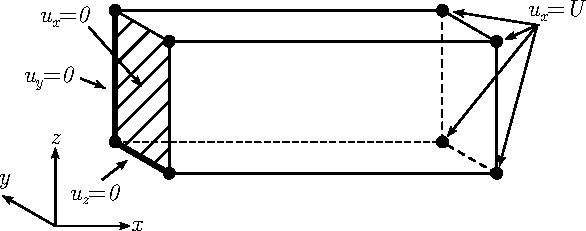
\includegraphics[width=0.8\linewidth]{tensileSetup.pdf}
    \caption[Displacement boundary conditions for dislocation plasticity modelling of single crystal, micro-tensile tests.]{Displacement boundary conditions for dislocation plasticity modelling of single crystal, micro-tensile tests.}
    \label{f:tensileSetupTop}
\end{figure}
Having dislocations exit those surfaces creates a slip step on them. This leads to very high stresses because the FEM essentially has to push the slip step back in order to make it conform to the displacement boundary conditions as in \cref{f:slipStep}, which is unphysical. In the bulk, they stop experiencing the Peach-K\"{o}hler force, because the bulk is not subject to the forces or displacements of the experiment, so dislocations tend to pile up, given the only forces they experience are from themselves and other dislocations.
\begin{figure}
    \centering
    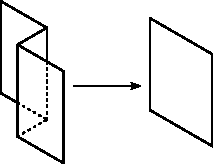
\includegraphics[width=0.5\linewidth]{slipStep.pdf}
    \caption{Slip step created by a dislocation exiting the volume has to be moved back to enforce displacement boundary conditions.}
    \label{f:slipStep}
\end{figure}

This was originally hard-coded for cantilever bending, but a general solution can be found with \cref{eq:signedDist},
\begin{align}\label{eq:signedDist}
    D & = \hat{\vec{n}} \cdot (\vec{x_0} - \vec{x_n})\,,
\end{align}
where $D$ is the signed distance from the point, $\vec{x_0}$, to a plane with unit normal, $\hat{\vec{n}}$, which passes through the point, $\vec{x_n}$. $D$ is positive if $\vec{x_0}$ is on the side $\hat{\vec{n}}$ points towards and negative otherwise. We can identify nodes that have exited from these surfaces by using their surface normal, a point on them, and whether $D$ is positive. They can then be moved back to the surface and pinned.

This is an imperfect solution, but works quite well and removes these nodes from the mobility calculation. Perhaps a better solution would be to flag those nodes such that Peach-K\"{o}ler forces, tractions, displacements, and surface remeshing criteria no longer apply to them. However, this will have to be implemented and tested as part of future improvements to the code.

\section{Conclusions}

Discrete dislocation dynamics is a stiff and chaotic dynamical system. It is very sensitive to small changes, as we will see in \cref{c:tractions}. Having a correct topology is of the utmost importance in this regard. Something as small as a collision that was not performed when it should have, can have dramatic downstream consequences. As dislocation density increases, the degree of correctness when resolving their interactions increases in importance. Not only does it increase the accuracy of a simulation, but improves its running speed.

The increase in accuracy is obvious; detecting all the collsions that should be detected; resolving them in a manner more keeping with the quasi-static assumption yielding the mobility law; and ensuring the network resolution is what it should be; make for more accurate simulations.

Part of the increase in running speed is down to the fact that quasi-static conditions are better met than before, so the timsetep can be greater. The other huge benefit to running speed is down to the asymptotic scaling and high scaling constants of the algorithms we use; $\mathcal{O}(N^2)$ for seg-seg forces and collisions; $\mathcal{O}(C!)$ for a single separation; $\mathcal{O}(M N)$ for tractions. Where $N$ is the number of segments, $C$ the number of connections, and $M$ the number of surface elements. Simply put, we disproportionately benefit from having fewer items these expensive functions operate over.

With these improvements, simulations that used to be computationally intractible within a reasonable timeframe are now very doable. Large, complex simulations with high dislocation densities are still slow by virtue of how topologically active they can be and due to the high cost of the remote forces, but they are simultaneously more accurate and faster by multiple orders of magnitude (sometimes 5 or more) than before.
\savearabiccounter
%3495 words